\documentclass[border=10pt]{standalone}
\usepackage{pgfplots}
\pgfplotsset{compat=1.18}
\begin{document}
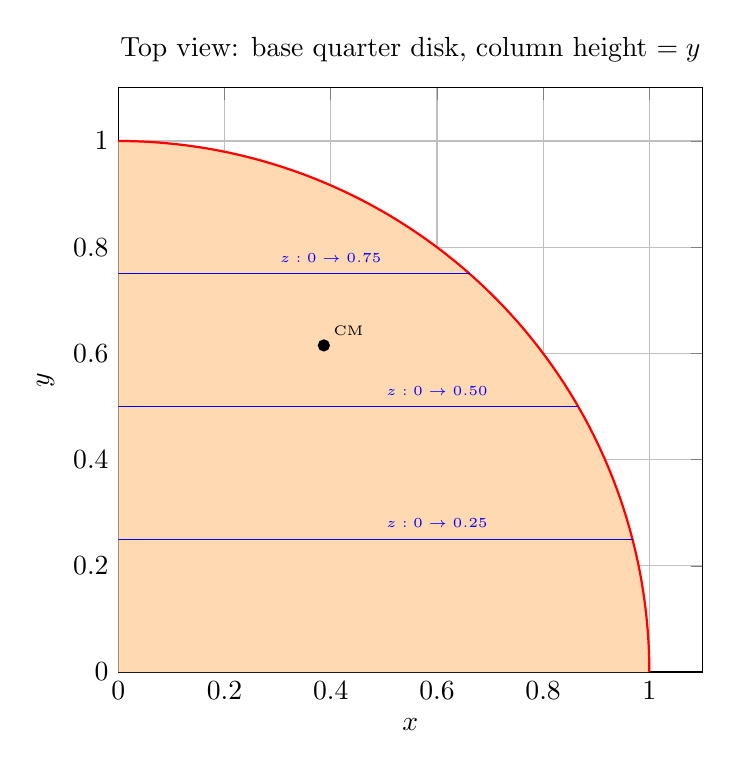
\begin{tikzpicture}
\begin{axis}[
    xlabel=$x$, ylabel=$y$,
    width=9cm,height=9cm,
    xmin=0,xmax=1.1,ymin=0,ymax=1.1,
    axis equal image,
    grid=both,
    trig format plots=deg,
    title={Top view: base quarter disk, column height $=y$}]
% quarter disk projection (filled)
\addplot[fill=orange!30, draw=none, domain=0:90, samples=100]
   ({cos(x)},{sin(x)}) -- (axis cs:0,0) -- cycle;
% boundary arc
\addplot[red, thick, domain=0:90, samples=100]({cos(x)},{sin(x)});
% rays at constant y : z runs 0 -> y
\addplot[blue,thin] coordinates {(0,0.25)(0.9682458,0.25)};
\addplot[blue,thin] coordinates {(0,0.50)(0.8660254,0.50)};
\addplot[blue,thin] coordinates {(0,0.75)(0.6614378,0.75)};
\node[blue,font=\tiny] at (axis cs:0.60,0.28){$z:0\to0.25$};
\node[blue,font=\tiny] at (axis cs:0.60,0.53){$z:0\to0.50$};
\node[blue,font=\tiny] at (axis cs:0.40,0.78){$z:0\to0.75$};
\addplot[only marks, mark=*, mark size=2pt] coordinates {(0.387,0.615)};
\node at (axis cs:0.387,0.615)[above right,font=\tiny]{CM};
\end{axis}
\end{tikzpicture}
\end{document}